\documentclass[11pt,letterpaper]{article}
\usepackage[utf8]{inputenc}
\usepackage{geometry}
\geometry{top=1in, bottom=1in, left=1in, right=1in}
\usepackage{amsmath}
\usepackage{amsfonts}
\usepackage{amssymb}
\usepackage{booktabs}
\usepackage{longtable}
\usepackage{tabularx} 
\usepackage{authblk}
\usepackage{graphicx}
\usepackage{lettrine}
\usepackage{hyperref}

% Set line spacing to 1.15 for better readability
\linespread{1.15}

% Custom column type definitions for clean wrapping and alignment inside tables
\newcolumntype{Y}{>{\centering\arraybackslash}X}
\newcolumntype{L}{>{\raggedright\arraybackslash}X}

% Adjust abstract look to match professional engineering style
\renewenvironment{abstract}
 {\small\quotation\bfseries\noindent\abstractname:\ }
 {\endquotation}

\title{\textbf{Development of an AI-Enhanced High-Fidelity Hybrid Semi-Symplectic Computational Framework for Massive Space Debris Fragmentation and Orbital Population Dynamics}}

\author{Juan Francisco Puerta-Ibarra\thanks{Lecturer and Ph.D. Candidate, Department of Mechanical and Aerospace Engineering.}}
\author{Nicolás Muñoz-Galeano\thanks{Professor, Research Group in Efficient Energy Management (GIMEL), Department of Electrical Engineering.}}
\author{Bonnie Prado Pino\thanks{Adjunct Professor, Department of Mechanical and Aerospace Engineering; Design Engineer at Odyssey Space Research, Houston, TX, 77058, USA.}}
\affil{Universidad de Antioquia, Medellín, Antioquia, 050010, Colombia}

\date{}

\begin{document}

\maketitle

\begin{abstract}
The exponential proliferation of anthropogenic space debris within Low Earth Orbit (LEO) presents an existential hazard to spatial operational sustainability. Deterministic multi-decade forecasting of massive fragmentation clouds is severely bottlenecked by traditional numerical integration architectures, which exhibit systemic numerical error accumulation and artificial secular energy drift. This doctoral research addresses the scalability and physical realism challenge by engineering and validating an AI-enhanced, high-fidelity, hybrid semi-symplectic computational framework\cite{rein_rebound_2012}. Building upon a verified geopotential baseline that couples a generalized symplectic library with the WHFast symplectic engine, this project implements a second-order Strang splitting sequence to mathematically integrate non-conservative environmental perturbations---specifically atmospheric drag and Solar Radiation Pressure (SRP)---without violating the underlying symplectic geometry of conservative gravitational flows. The numerical architecture enforces physical conservation laws during large-scale simulations up to 50,000 individual fragments\cite{tamayo_reboundx_2020}. To transcend current scaling limitations and operationalize real-time tracking, the subsequent phase integrates three distinct artificial intelligence tiers: Physics-Informed Neural Networks (PINNs) as surrogate thermospheric weather models, Deep Learning architectures (LSTMs/Transformers) for automated macro-scale conjunction mapping, and Reinforcement Learning (RL) agents optimized for autonomous bidirectional event reconstruction. This framework provides academic, regulatory, and industrial aerospace stakeholders with a scalable, highly accurate predictive tool crucial for orbital traffic coordination and space sustainability policy enforcement.
\end{abstract}

\section*{Nomenclature}

\begin{longtable}{@{}l @{\quad=\quad} l@{}}
$\mathbf{a}_{\text{grav}}$ & gravitational acceleration vector, $\text{m/s}^2$ \\
$\mathbf{a}_{\text{drag}}$ & atmospheric drag perturbation acceleration vector, $\text{m/s}^2$ \\
$\mathbf{a}_{\text{SRP}}$  & solar radiation pressure perturbation acceleration vector, $\text{m/s}^2$ \\
$H_{\infty}$               & modified or shadowed numerical Hamiltonian operator \\
$h$                        & instantaneous geocentric altitude base, $\text{m}$ \\
$H$                        & height-dependent atmospheric scale factor, $\text{m}$ \\
$\rho$                     & local thermospheric mass density field, $\text{kg/m}^3$ \\
$\rho_0$                   & nominal base atmospheric reference value, $\text{kg/m}^3$ \\
$C_D$                      & non-dimensional aerodynamic drag structure coefficient \\
$A/m$                      & specific structural area-to-mass ratio parameter, $\text{m}^2/\text{kg}$ \\
$P_{\text{SRP}}$           & solar radiation constant pressure factor, $\text{N/m}^2$ \\
$q$                        & non-dimensional specular material reflectivity metric \\
$\hat{\mathbf{r}}_{\text{sun}}$ & unit line-of-sight vector mapping the geocentric position of the Sun \\
$\Phi_G$                   & conservative gravitational flow transformation sub-operator \\
$\Phi_P$                   & non-conservative perturbative mapping displacement operator \\
$\Delta t$                 & constant layout discrete integration step size interval, $\text{s}$ \\
$L_c$                      & characteristic fragment dimension length metric, $\text{m}$ \\
$M_e$                      & total net mass generated during a collisional breakup event, $\text{kg}$
\end{longtable}


\section{Introduction and Problem Statement}
\lettrine{T}{he} contemporary ``NewSpace'' era is driving an unprecedented deployment of commercial mega-constellations, rapidly steering Low Earth Orbit (LEO) toward a critical saturation threshold. Recent census assessments indicate that there are currently more than 31,000 to 35,000 orbital objects larger than 10 cm tracked by global surveillance networks, alongside an untrackable population exceeding 500,000 fragments larger than 1 cm capable of causing catastrophic kinetic destruction upon impact. Historical metrics compiled within global registries highlight that the major catalysts for this debris field are propulsion-related staging malfunctions (29\%), anomalous space detachments (22\%), undocumented breakup configurations (20\%), and deliberate hypervelocity kinetic anti-satellite (ASAT) engagements (11\%).\cite{european_space_agency_space_nodate}\cite{anz-meador_assessment_2004}\cite{kessler_collision_1978}

\begin{figure}[hbt!]
\centering
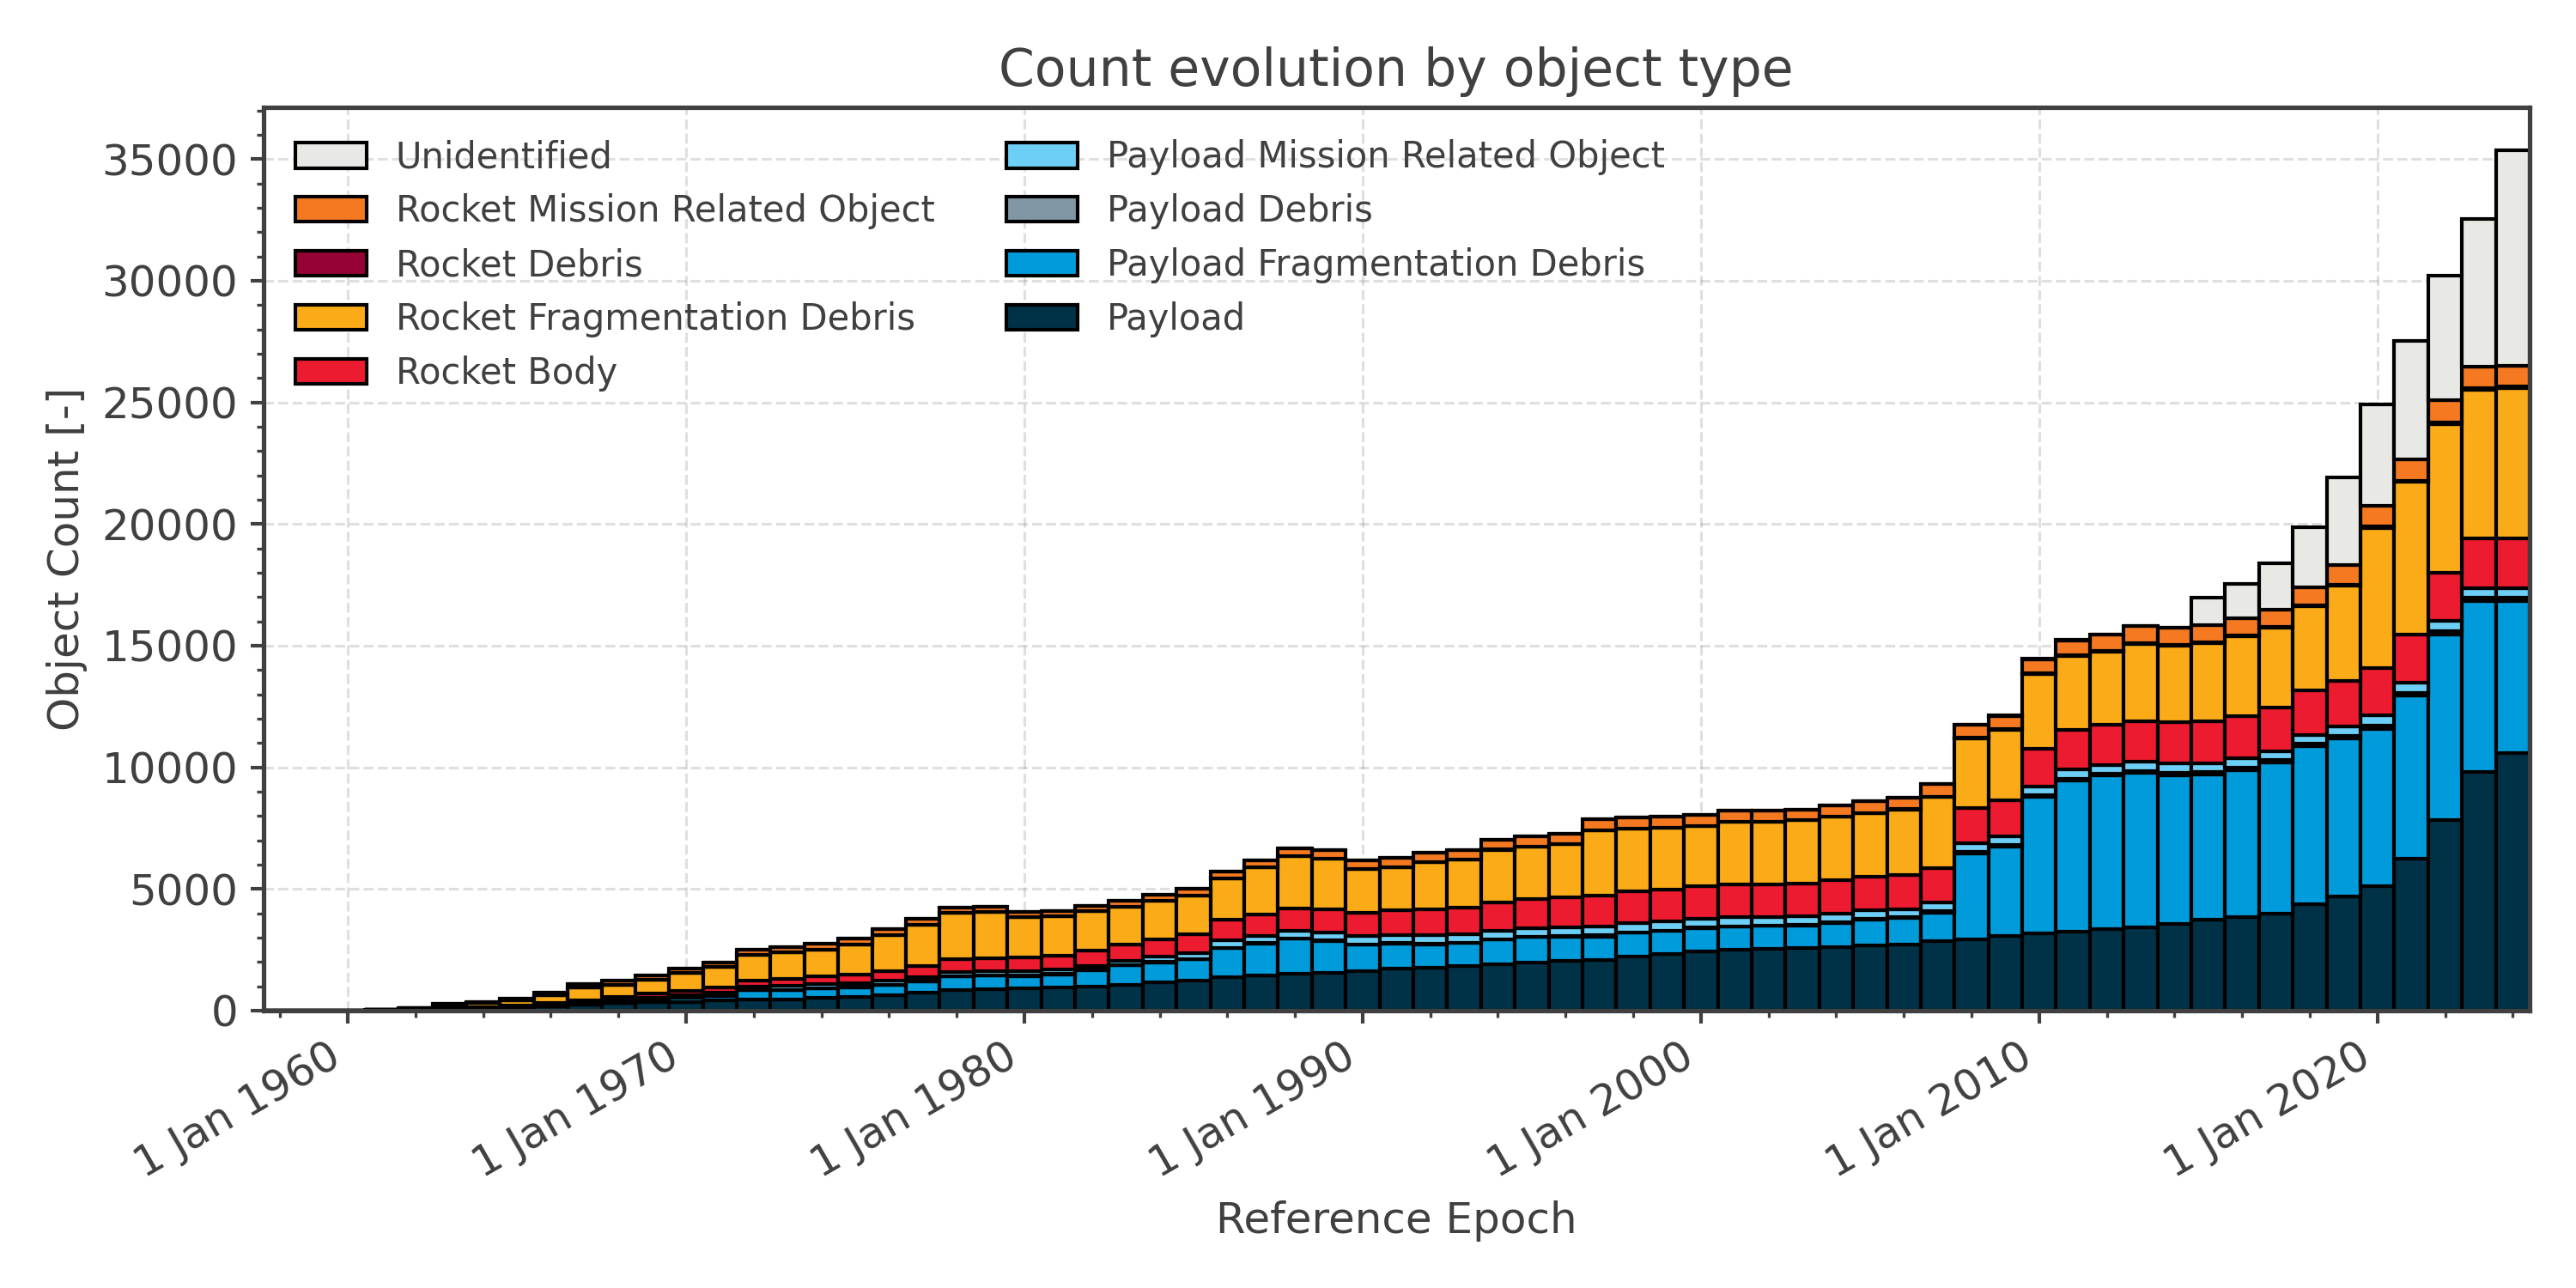
\includegraphics[width=1\linewidth]{allEvoTypeCnt.png}
\caption{Historical trend of fragment propagation in near-Earth orbits from 1957 to present-day projections.}
\label{fig:debris_timeline}
\end{figure}

The fundamental scientific challenge resides in the long-term, multi-decade forecasting of the evolutionary pathways of massive fragment clouds with strict physical integrity\cite{letizia_analytical_2014}. When a catastrophic fragmentation occurs---such as the landmark 2007 Fengyun-1C ASAT event or the 2009 Iridium-Cosmos hypervelocity collision---thousands of long-lived fragments are immediately dispersed into highly dynamic trajectories\cite{matney_measurements_2008}\cite{wang_analysis_2010}. Traditional mission planning orbit propagators fail under massive tracking scenarios due to two primary algorithmic bottlenecks:

\begin{figure}[hbt!]
\centering
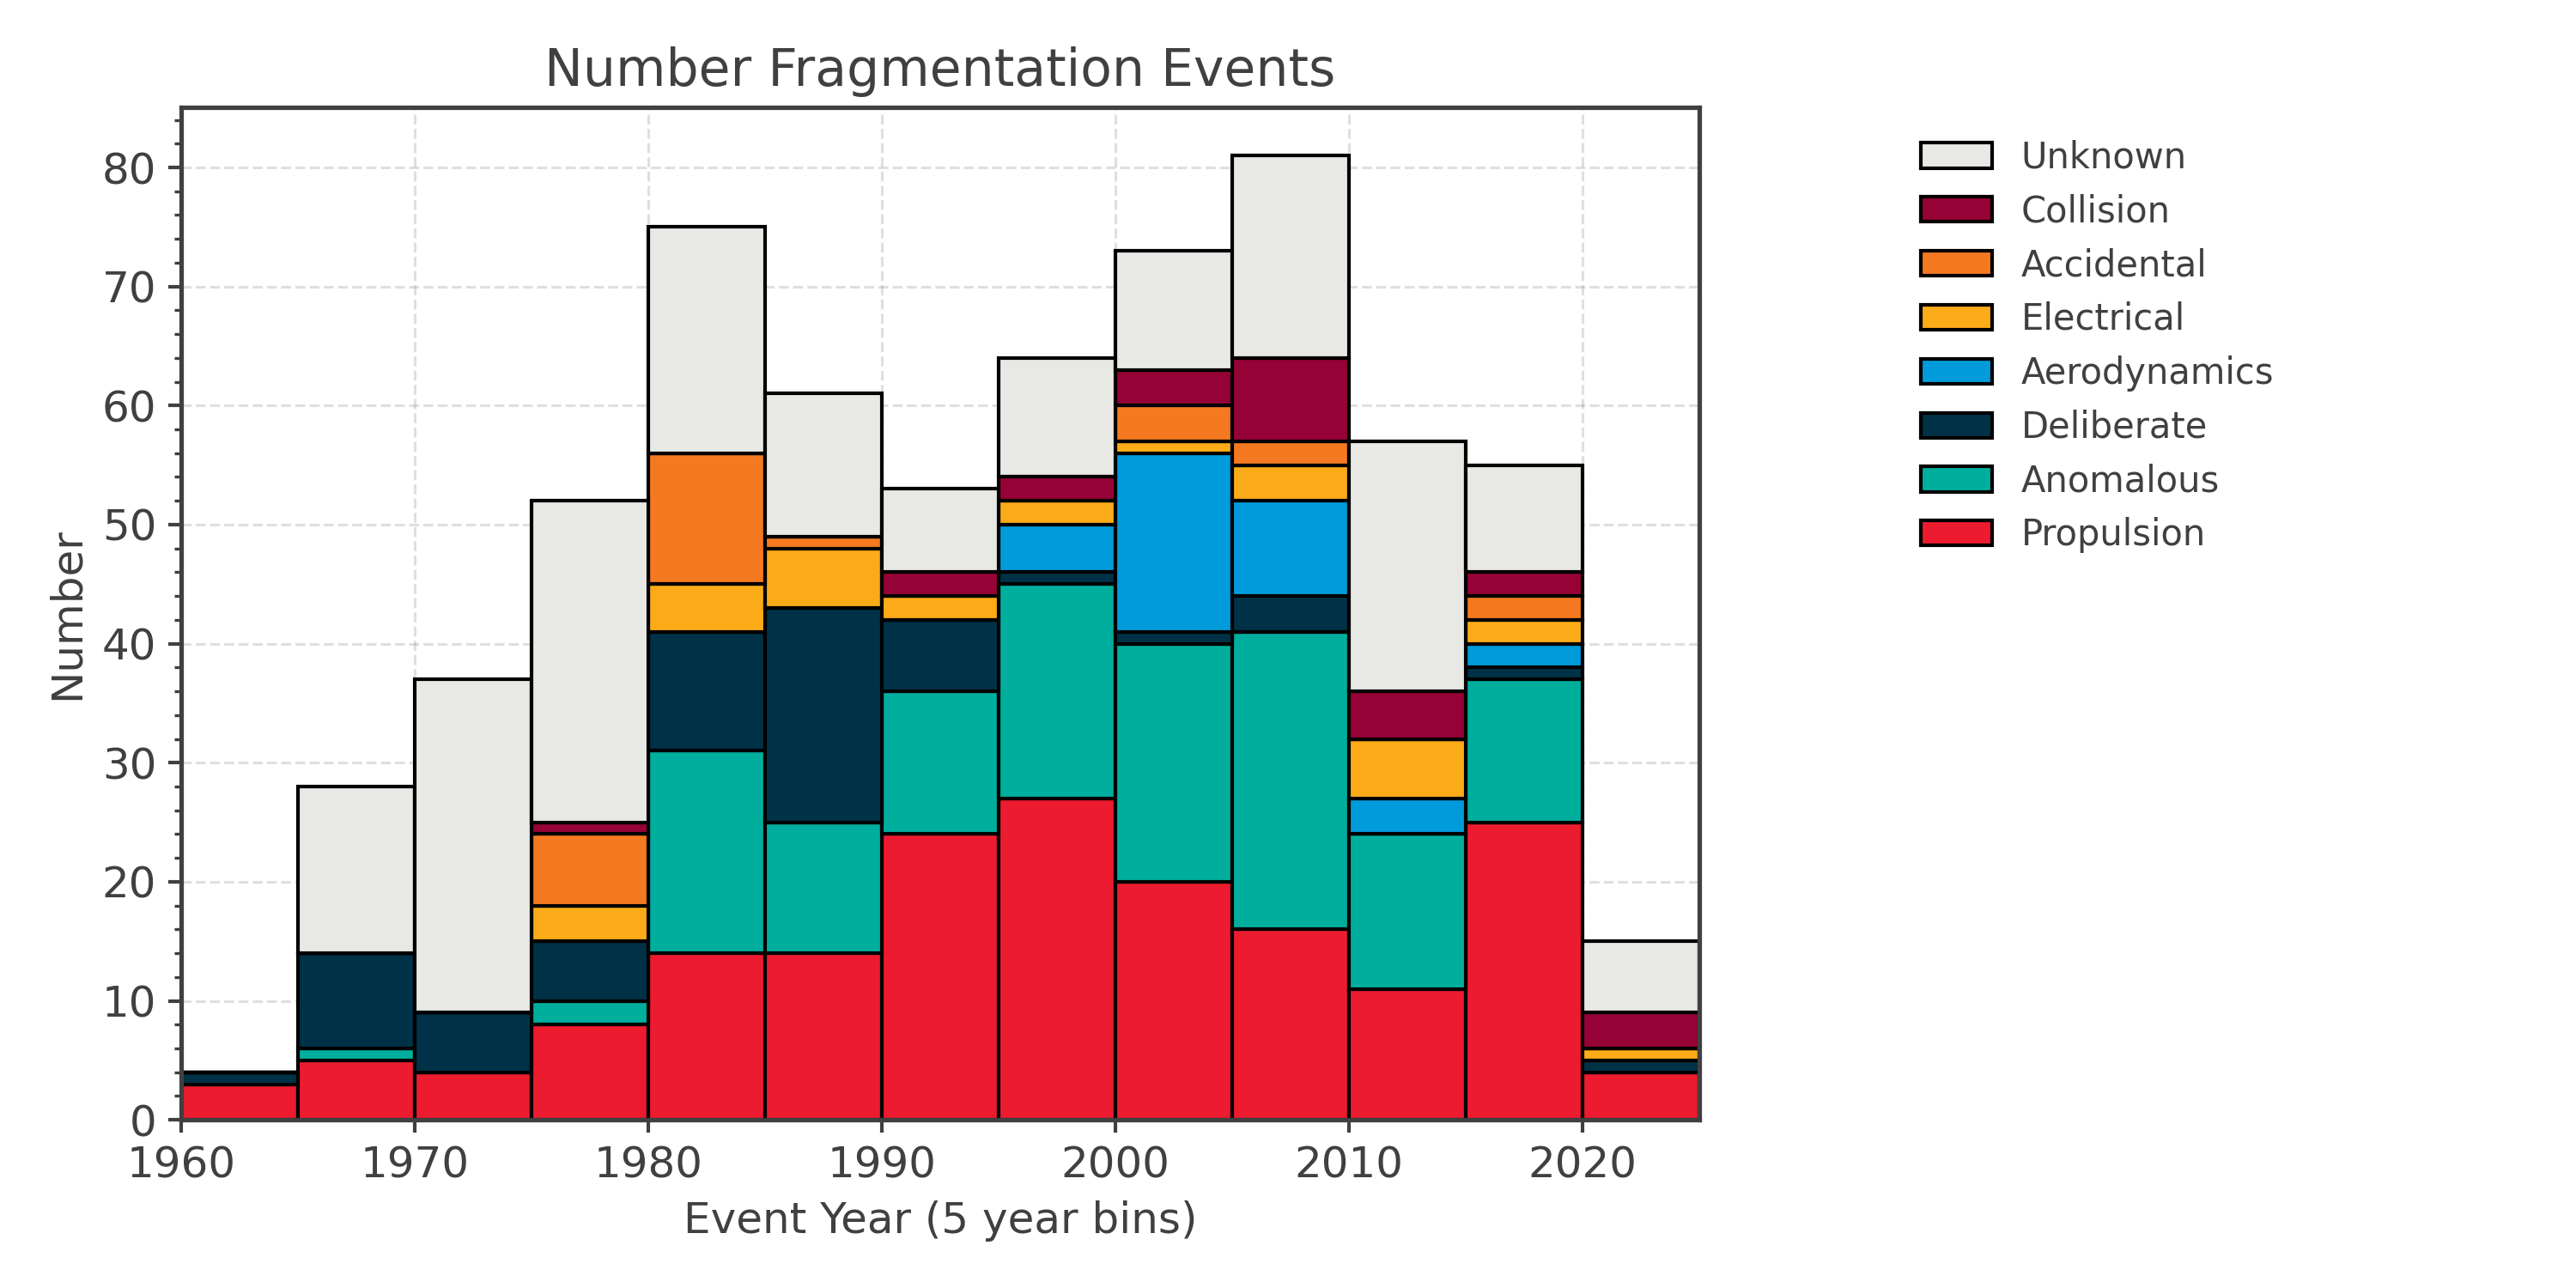
\includegraphics[width=1\linewidth]{eventCausesPerEY_abs.png}
\caption{Statistical breakdown of spacecraft breakup triggers cataloged within the European Space Agency's (ESA) Fragmentation Database.}
\label{fig:esa_pie_chart}
\end{figure}

\begin{enumerate}
    \item \textbf{Computational Scalability Bottleneck:} Standard integration methods propagate objects sequentially, creating a linear computational overhead ($\mathcal{O}(N)$) that renders large-population cloud analyses ($N > 10,000$) computationally unviable over multi-year regimes.
    \item \textbf{Numerical Dissipation Drift:} Classical high-order explicit numerical schemes (e.g., Runge-Kutta, Prince-Dormand, or direct Cowell implementations) introduce non-physical truncation errors that systematically accumulate over multi-decade cycles. This accumulation causes an artificial secular drift in the system's total mechanical energy, resulting in false contractions or expansions of predicted orbital boundaries.
\end{enumerate}


\section{Theoretical Framework and State of the Art}
The mathematical modeling of orbital environments requires separating the underlying physical forces into conservative Hamiltonian potentials and non-conservative environmental perturbations\cite{luo_applying_2017}\cite{sanz-serna_symplectic_1992}. Traditional celestial mechanics relies heavily on explicit numerical integrations like Cowell's method, which solves Newton’s second law directly:
\begin{equation}
    \dot{\mathbf{v}} = \mathbf{a}_{\text{grav}} + \sum_{i} \mathbf{a}_{\text{i}}
\end{equation}
where $\mathbf{a}_{\text{grav}}$ encompasses central point-mass dynamics alongside the non-spherical geopotential zonal harmonics ($J_2, J_4$), and $\mathbf{a}_{i}$ accounts for non-conservative perturbations such as atmospheric drag and solar radiation pressure. Alternate analytical approaches like Encke's method or Gauss's variation of parameters refine local step stability but remain limited when modeling chaotic, high-density fragmentation envelopes.

\begin{figure}[hbt!]
\centering
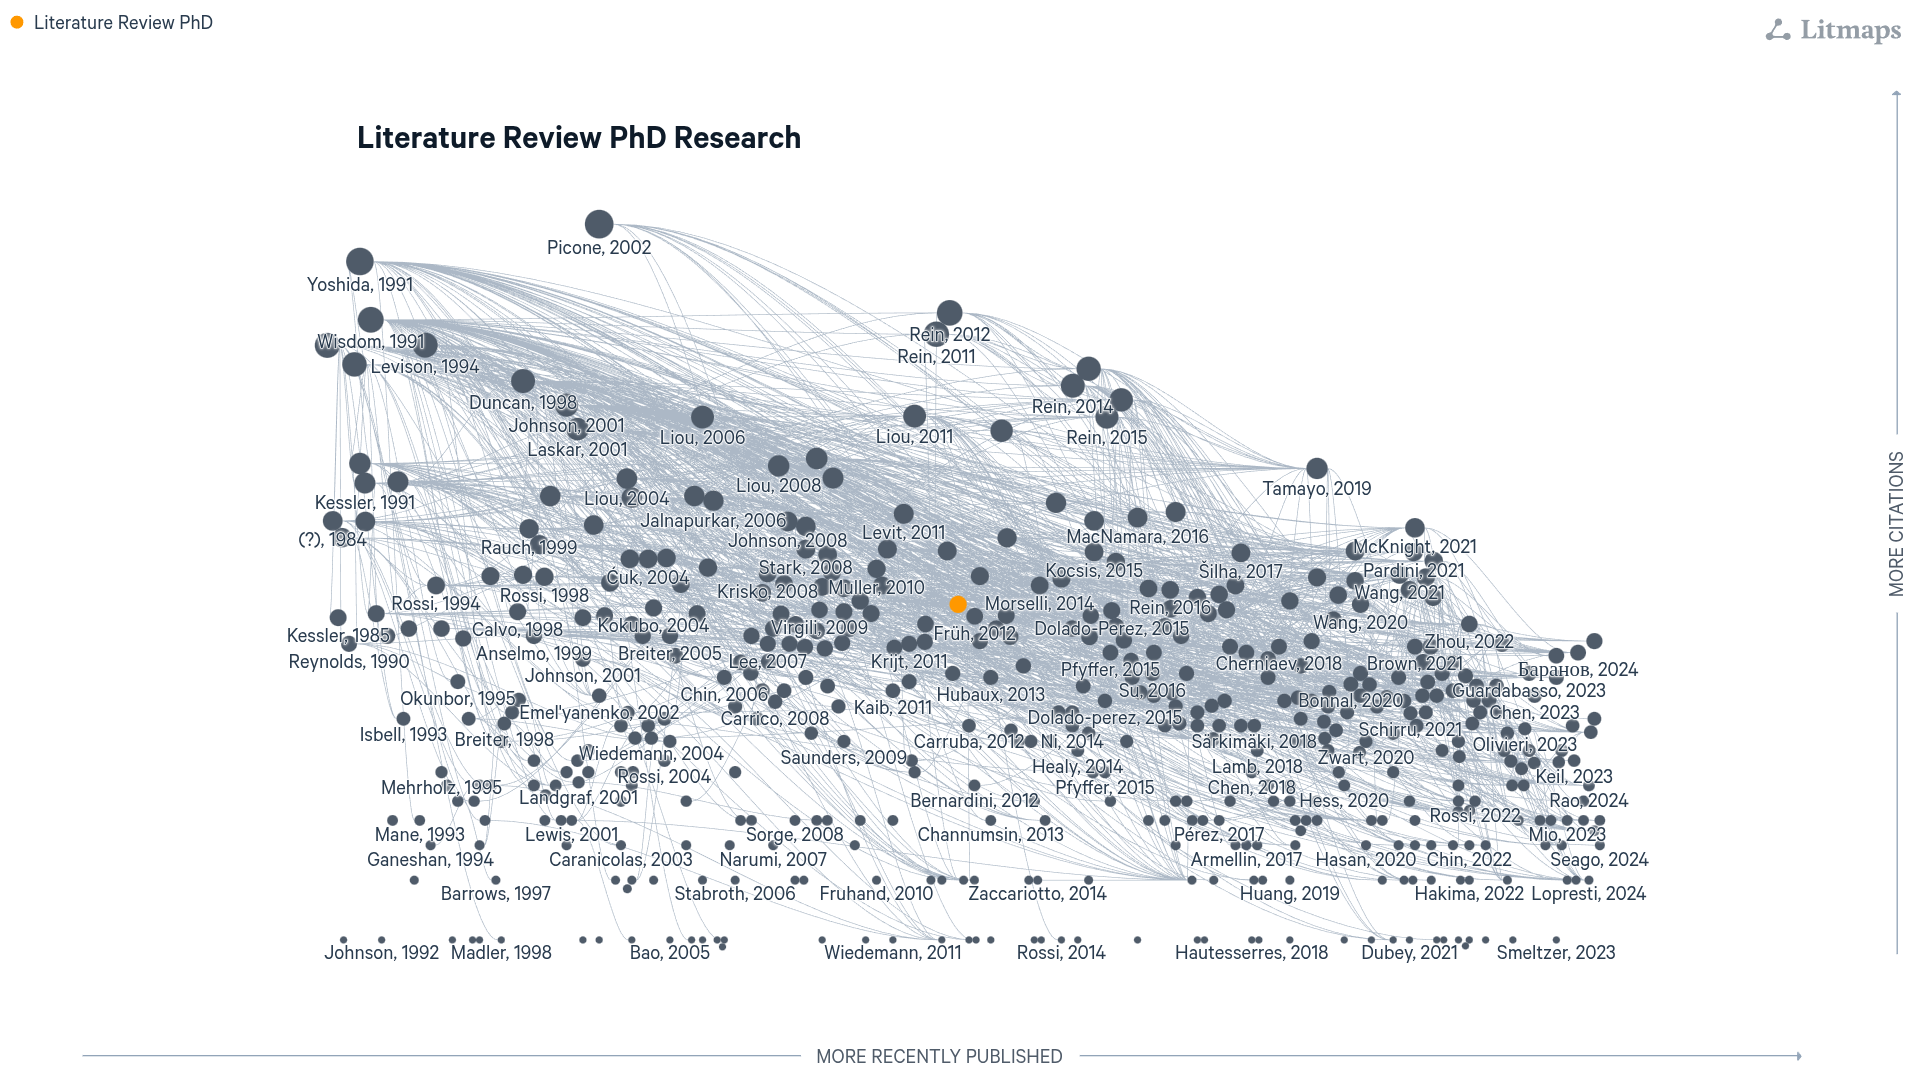
\includegraphics[width=1\linewidth]{LitmapMap.png}
\caption{Citation mapping and network cluster distribution outlining foundational literature landmarks in long-term astrodynamics and symplectic development.}
\label{fig:litmaps_network}
\end{figure}

To mitigate numerical error growth, symplectic integrators have been introduced\cite{tsang_slimplectic_2015}. Grounded in backward error interpretation, a symplectic mapping applied to a Hamiltonian system simulates a nearby modified Hamiltonian system exactly:
\begin{equation}
    H_{\infty} = H + \mathcal{O}(h^r)
\end{equation}
Because the computed state vectors remain bounded to the phase-space manifolds of $H_{\infty}$, symplectic algorithms effectively eliminate artificial secular energy drift, ensuring high qualitative accuracy over planetary scales.

Hubaux et al. demonstrated that modeling space debris in LEO introduces non-Hamiltonian dissipative forces that violate standard symplectic conservation axioms. Atmospheric drag operates directly opposite to the velocity vector:
\begin{equation}
    \mathbf{a}_{\text{drag}} = -\frac{1}{2}\frac{C_D A}{m} \rho(v) v \mathbf{v}
\end{equation}
where $C_D$ is the drag coefficient, $A/m$ is the specific area-to-mass ratio, and $\rho(v)$ represents the local thermospheric density characterized by advanced height-dependent scale heights ($H$):
\begin{equation}
    \rho(h) = \rho_0 \exp\left(-\frac{h - h_0}{H}\right)
\end{equation}
Concurrently, Solar Radiation Pressure injects continuous perturbation vectors modeled as:
\begin{equation}
    \mathbf{a}_{\text{SRP}} = -P_{\text{SRP}} \frac{A_{\text{SRP}}}{m} (1+q) \hat{\mathbf{r}}_{\text{sun}}
\end{equation}
where $P_{\text{SRP}}$ represents the solar pressure constant, $q$ is the specular reflectivity, and $\hat{\mathbf{r}}_{\text{sun}} $ is the geocentric Sun unit vector.

The current state of the art resolves this intersection via operator splitting methodologies\cite{macnamara_operator_2016}. By executing a symmetric, second-order Strang splitting sequence, the net evolution operator $\Phi(\Delta t)$ separates into non-interacting conservative ($\Phi_G$) and non-conservative ($\Phi_P$) integration flows:
\begin{equation}
    \Phi(\Delta t) \approx \Phi_P\left(\frac{\Delta t}{2}\right) \circ \Phi_G(\Delta t) \circ \Phi_P\left(\frac{\Delta t}{2}\right)
\end{equation}
The baseline architecture established in previous years coupled the chosen symplectic library framework with the WHFast solver, demonstrating sub-kilometer spatial cross-verification with NASA's GMAT for a 20,000-object geopotential-only cloud\cite{noauthor_general_nodate-1}. Recent developments advanced this baseline by demonstrating that a constant step-size ($\Delta t = 10$~s) hybrid Strang integration can reliably track 50,000 objects over annual cycles with a 0.005\% agreement in analytical nodal precession. 

The critical research gap now lies in the fact that while this hybrid scheme maintains a highly scalable power-law performance exponent of 1.60, a full one-year propagation still requires 18 days of dedicated workstation execution. To make this architecture viable for real-time space situational awareness, surrogate AI frameworks must be integrated to bypass heavy computational bottlenecks.


\section{Project Objectives}

\subsection{General Objective}
To develop, validate, and optimize an AI-enhanced high-fidelity hybrid semi-symplectic computational framework capable of modeling massive space debris fragmentation and long-term population dynamics within non-conservative orbital environments to support space traffic management and sustainability operations.

\subsection{Specific Objectives and Verifiable Indicators}
\begin{enumerate}
    \item \textbf{Objective 1:} Implement and mathematically verify a second-order Strang splitting integration scheme that couples high-order geopotential models with non-conservative perturbations (piecewise-exponential atmospheric drag and solar radiation pressure).
    \begin{itemize}
        \item \emph{Indicator 1.1:} Preservation of numerical energy error bounds within a strict $|\Delta E / E_0| \in [10^{-8}, 10^{-7}]$ baseline during long-duration cycles.
        \item \emph{Indicator 1.2:} Relative error of secular nodal precession is restricted below 0.005\% when validated against analytical orbital mechanics theory.
    \end{itemize}
    \item \textbf{Objective 2:} Scale the parallel computing capacity of the semi-symplectic C-based implementation to seamlessly process high-density debris environments exceeding 50,000 autonomous fragments.
    \begin{itemize}
        \item \emph{Indicator 2.1:} Empirical verification of an execution scalability profile adhering to a power-law exponent of approximately 1.60.
        \item \emph{Indicator 2.2:} Computational observation of the ``orbital sorting'' effect, successfully segregating high area-to-mass ratio fragments ($>0.05~\text{m}^2/\text{kg}$) over annual cycles.
    \end{itemize}
    \item \textbf{Objective 3:} Integrate specialized deep learning architectures and physics-informed neural networks to eliminate computational latency in conjunction with forecasting and thermospheric modeling.
    \begin{itemize}
        \item \emph{Indicator 3.1:} Training and execution of a PINN thermospheric surrogate capable of generating local density values matching piecewise exponential reference profiles while lowering computation times.
        \item \emph{Indicator 3.2:} Execution of an automated Transformer/LSTM tracking mechanism that screens the 50,000-particle cloud to identify high-probability conjunctions in real time.
    \end{itemize}
\end{enumerate}


\section{Methodology}
The compressed research workflow is structured into four sequential technical execution phases designed to fulfill each specific project objective over a 2-year duration (24 months):

\begin{figure}[hbt!]
\centering
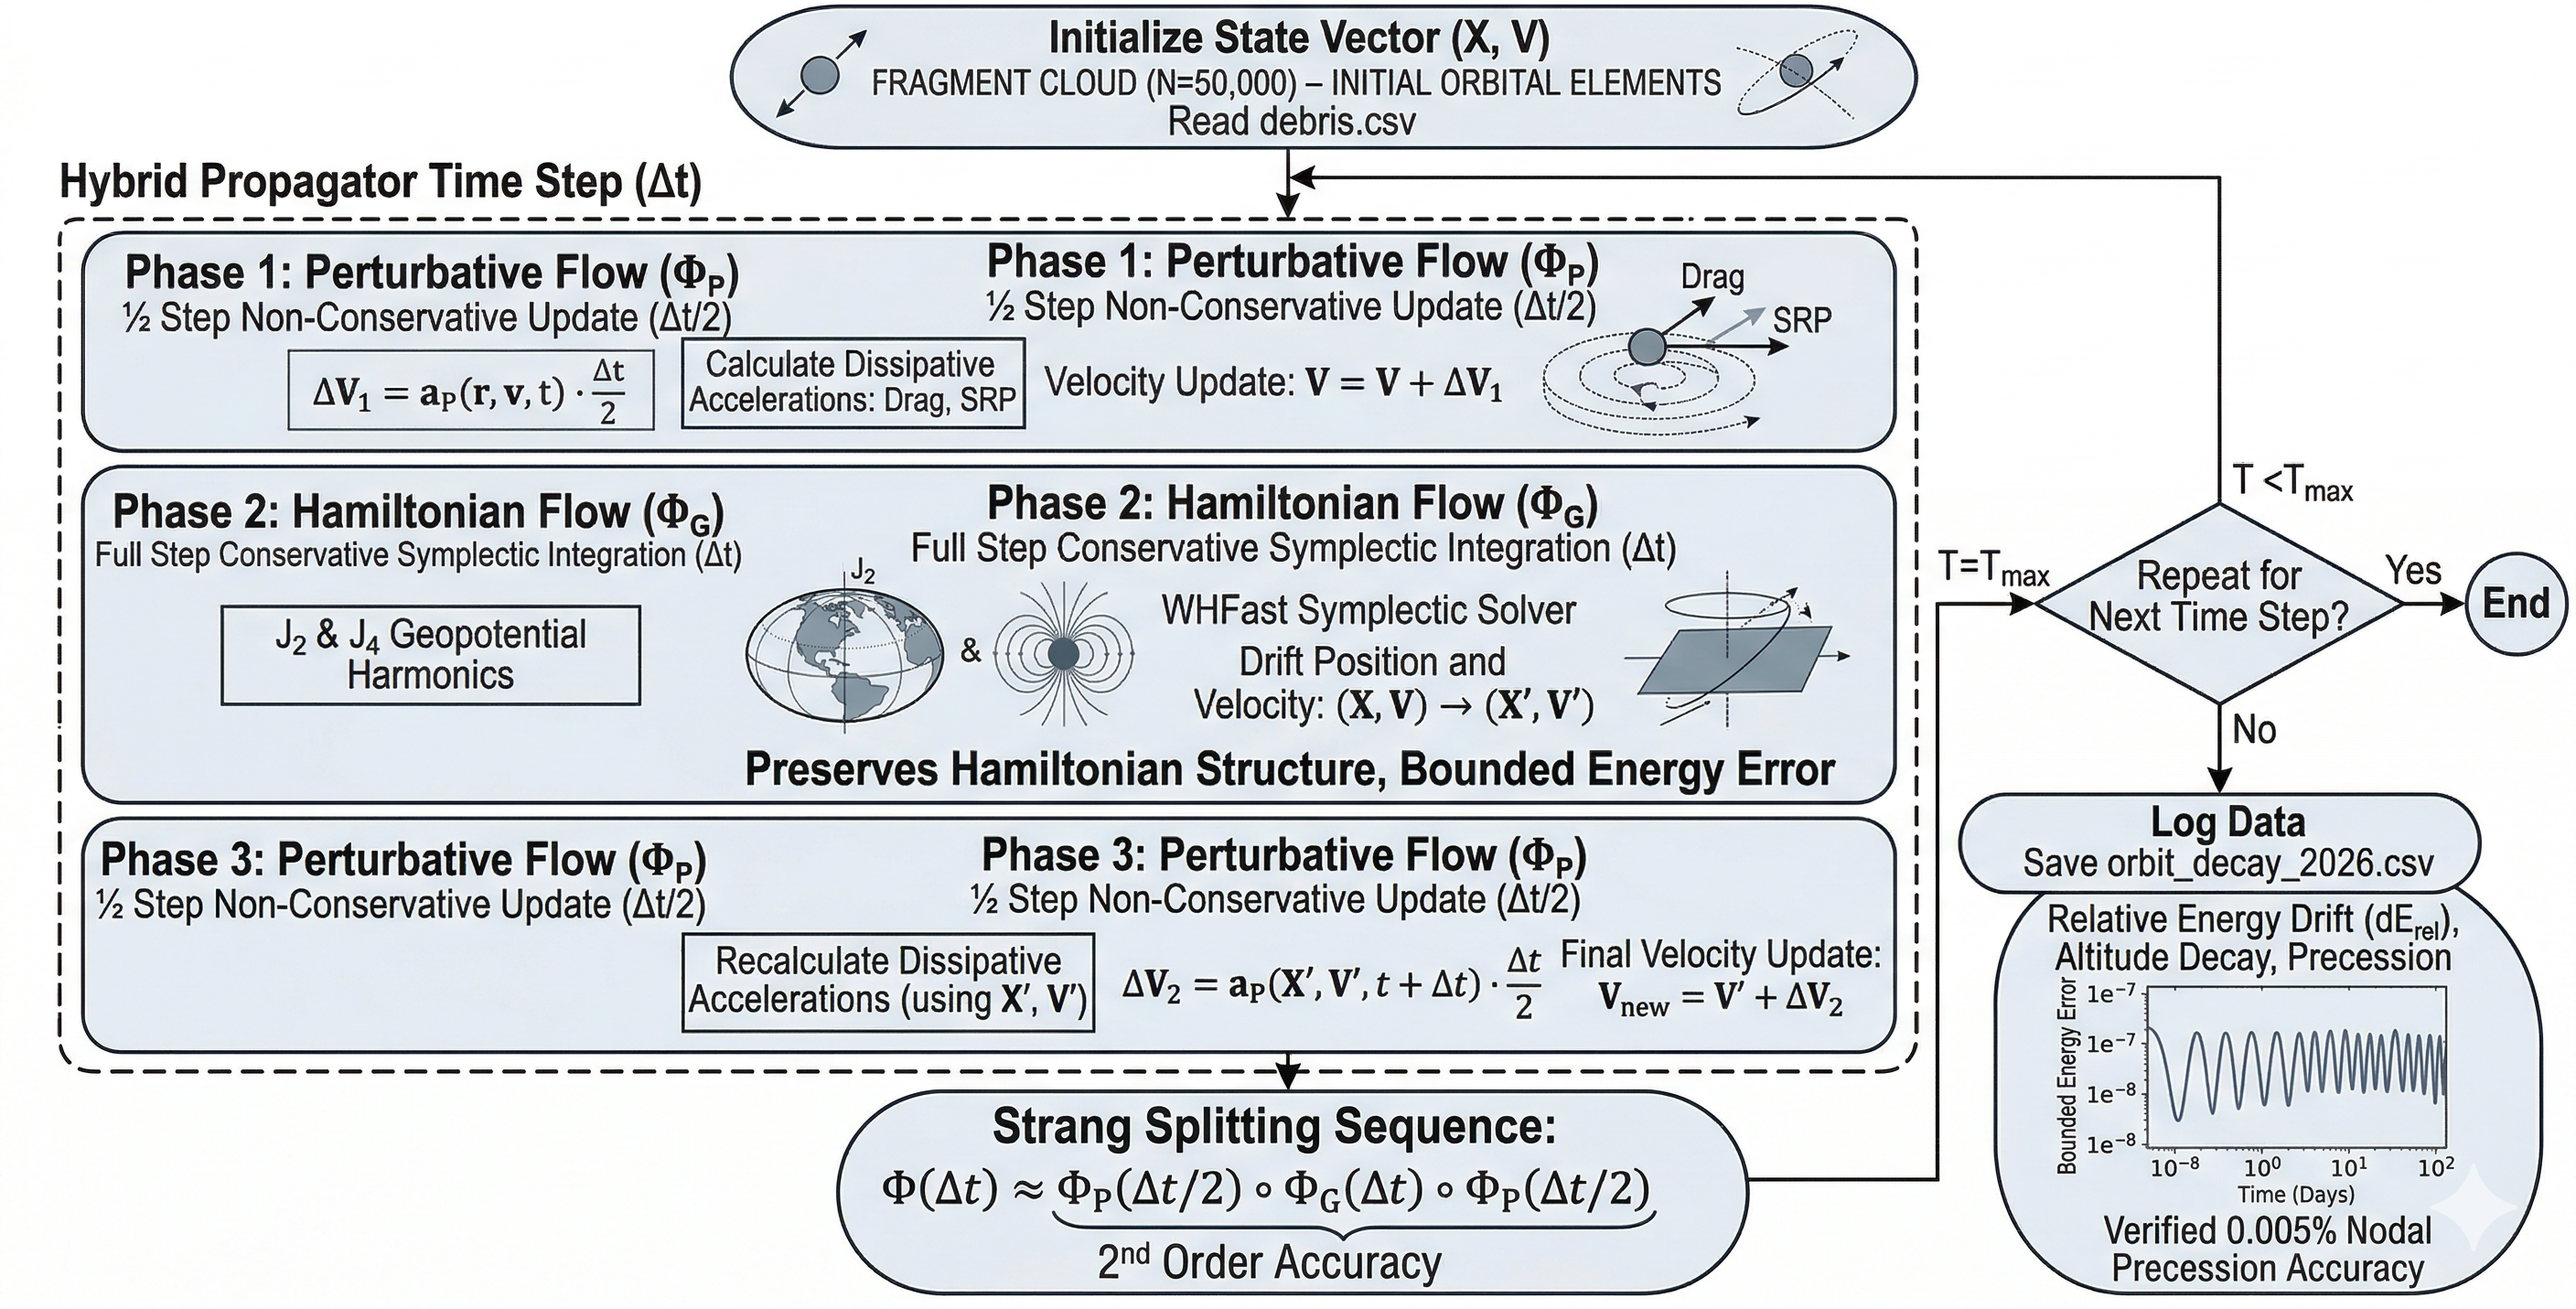
\includegraphics[width=1\linewidth]{splitting_flowchart_v2.png} 
\caption{Detailed multi-phase algorithmic flowchart outlining the implementation steps of the second-order symmetric Strang splitting loop.}
\label{fig:strang_flowchart}
\end{figure}

\subsubsection*{Phase 1: Hybrid Integrator Formulation and Environmental Force Coupling}
The numerical engine will build upon a foundational symplectic library architecture. We will explicitly implement the symmetric second-order Strang splitting sequence. Within a discrete constant time step ($\Delta t = 10$ s), the execution loop will operate via a discrete three-phase sequence:
\begin{enumerate}
    \item \textbf{First Perturbative Half-Step ($\Phi_P$):} Apply an analytical velocity correction vector over an interval of $\Delta t/2$ utilizing real-time non-conservative accelerations ($\mathbf{a}_{\text{drag}} + \mathbf{a}_{\text{SRP}}$) calculated from the structural profiles.
    \item \textbf{Full Hamiltonian Step ($\Phi_G$):} Advance the spatial state vector over the full interval $\Delta t$ using the WHFast symplectic solver, integrating the $J_2, J_4$ geopotential harmonics while bounding numerical truncation growth.
    \item \textbf{Second Perturbative Half-Step ($\Phi_P$):} Recompute the dissipative environmental accelerations at the newly updated state vector and apply a final velocity correction over $\Delta t/2$.
\end{enumerate}

\subsubsection*{Phase 2: Scale Optimization and Orbital Sorting Analysis}
The fragment population will be expanded to 50,000 objects utilizing randomized but physically bounded LEO orbital elements (altitude $400 - 1000$ km, eccentricity $0 - 0.05$, inclination $0^\circ - 100^\circ$). The simulation engine will incorporate mass and momentum conservation subroutines derived from NASA's Standard Breakup Model architecture to mathematically initialize fragment distribution fields ($L_c, A/m, \Delta v$)\cite{johnson_nasas_2001}. Computational profiling scripts will run continuously to verify that multi-core CPU scaling preserves the theoretical power-law performance slope of 1.60. Long-term runs will be cataloged to monitor the orbital sorting divergence driven by varied area-to-mass distributions.

\begin{figure}[hbt!]
\centering
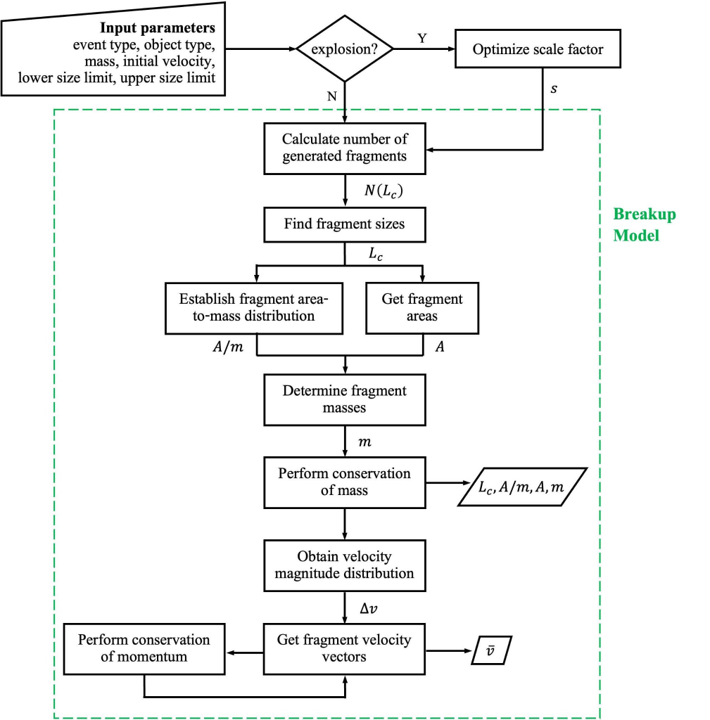
\includegraphics[width=1\linewidth]{NSBM_Ariel.png} 
\caption{Algorithmic workflow structure of the integrated Standard Breakup Model (SBM) mapping particle property distributions under strict physical constraints.\cite{black_decluttering_2024}}
\label{fig:nasa_sbm_flowchart}
\end{figure}

\subsubsection*{Phase 3: Artificial Intelligence Core Integration}
To accelerate the computational timeline, three specific AI architectures will be integrated directly into the semi-symplectic C-loop:
\begin{itemize}
    \item \textbf{PINN Space Weather Surrogate:} A Physics-Informed Neural Network will be trained to map local altitude profiles directly to thermospheric density values ($\rho$), using the continuous physical equations of hydrostatic equilibrium as loss function regularization weights to substitute for grid-based exponential routines\cite{wu_investigation_2023}.
    \item \textbf{Deep Learning Conjunction Predictor:} Long Short-Term Memory (LSTM) networks or compact Transformer blocks will be trained on the aggregate historical particle state vectors to predict closing distances between fragments and active payloads, establishing real-time collision flags.
    \item \textbf{Reinforcement Learning Event Reconstructor:} Deep Q-Networks or Actor-Critic agents will be deployed to automate backward orbital propagation regimes, dynamically determining unknown parent satellite break-up coordinates from sparse telemetry profiles.
\end{itemize}

\subsubsection*{Phase 4: Comparative Benchmarking and Validation}
The finalized AI-enhanced architecture will undergo strict verification against industry benchmarks. A statistical subset of the simulated fragment clouds will be cross-propagated using NASA's General Mission Analysis Tool (GMAT) under identical physical parameters to verify sub-kilometer positional agreement. Final validation metrics will require secular orbital element oscillations to remain strictly bounded with zero unmodeled directional drift across decadal tracking iterations.


\section{Project Execution Parameters}

\subsection{Project Timeline}
The comprehensive execution layout spans a 2-year doctoral trajectory (24 months). Milestone performance matrices are explicitly organized across discrete operational phases in Table~\ref{tab:cronograma}.

\begin{table}[h!]
\caption{Doctoral Research Phase and Milestone Development Timeline (2-Year Plan)}
\label{tab:cronograma}
\centering
\begin{tabularx}{\textwidth}{Lcccccc}
\hline
\textbf{Research Phase Descriptor} & \textbf{M1--M4} & \textbf{M5--M8} & \textbf{M9--M12} & \textbf{M13--M16} & \textbf{M17--M20} & \textbf{M21--M24} \\ \hline
1. Strang Splitting Integration Core & X & & & & & \\
2. Model Scaling to 50k Particles  & & X & & & & \\
3. PINN Thermospheric Code Training & & & X & & & \\
4. Conjunction LSTM/Transformer Logic & & & & X & & \\
5. Backward RL Path Reconstruction & & & & & X & \\
6. Cross-GMAT Verification \& Thesis & & & & & & X \\ \hline
\end{tabularx}
\end{table}

\subsection{Project Budget Configuration}
The global financial allocation tracking maps directly to the infrastructure profiles of the Faculty of Engineering at Universidad de Antioquia. The consolidated global values are detailed inside Table~\ref{tab:budget}, followed by specialized breakdowns inside Tables~\ref{tab:personnel} and \ref{tab:equipment}. These costs are subject to variations.

\begin{table}[h!]
\caption{Consolidated Global Budget (Values in Thousands of COP)}
\label{tab:budget}
\centering
\begin{tabularx}{\textwidth}{Lccc}
\hline
\textbf{Budget Item (Rubros)} & \textbf{GIMEL Research Group} & \textbf{External Funding Sources} & \textbf{Total Aggregated} \\ \hline
Personnel Expenses            & \$120,000                     & \$60,000                          & \$180,000                 \\
Equipment Infrastructure      & \$15,000                      & \$0                               & \$15,000                  \\
Software Implementations       & \$0                           & \$0                               & \$0                       \\
Field Logistics \& Travel     & \$5,000                       & \$8,000                           & \$13,000                  \\
Open-Access Publications      & \$4,000                       & \$4,000                           & \$8,000                   \\ \hline
\textbf{Total Funding}        & \textbf{\$144,000}            & \textbf{\$72,000}                 & \textbf{\$216,000}        \\ \hline
\end{tabularx}
\end{table}

\begin{table}[h!]
\caption{Detailed Personnel Dedication Allocation}
\label{tab:personnel}
\centering
\small
\begin{tabularx}{\textwidth}{lLLcY}
\hline
\textbf{Investigator / Role} & \textbf{Academic Degree} & \textbf{Project Function} & \textbf{Dedication} & \textbf{Total (COP)} \\ \hline
Juan F. Puerta-Ibarra     & M.Sc. Aerospace Eng.     & Primary Ph.D. Candidate   & 40 h/week           & \$120,000         \\
N. Muñoz-Galeano          & Ph.D. Electrical Eng.    & Principal Thesis Director & 8 h/week            & \$120,000          \\
Bonnie Prado Pino         & Ph.D. Aerospace Eng.     & External Advisor          & 2 h/week            & \$120,000          \\ \hline
\end{tabularx}
\end{table}

\begin{table}[h!]
\caption{Technical Equipment Asset Registration}
\label{tab:equipment}
\centering
\begin{tabularx}{\textwidth}{lLLr}
\hline
\textbf{Equipment Descriptor} & \textbf{Operational Justification} & \textbf{Resource Type} & \textbf{Total Cost} \\ \hline
Multi-Core CPU Workstation    & 50k fragment cloud simulation loops & Direct Purchase & \$15,000            \\
Personal Computer Terminal       & Local compilation \& debugging      & Existing Asset  & \$0                 \\ \hline
\end{tabularx}
\end{table}


\begin{figure}[hbt!]
\centering
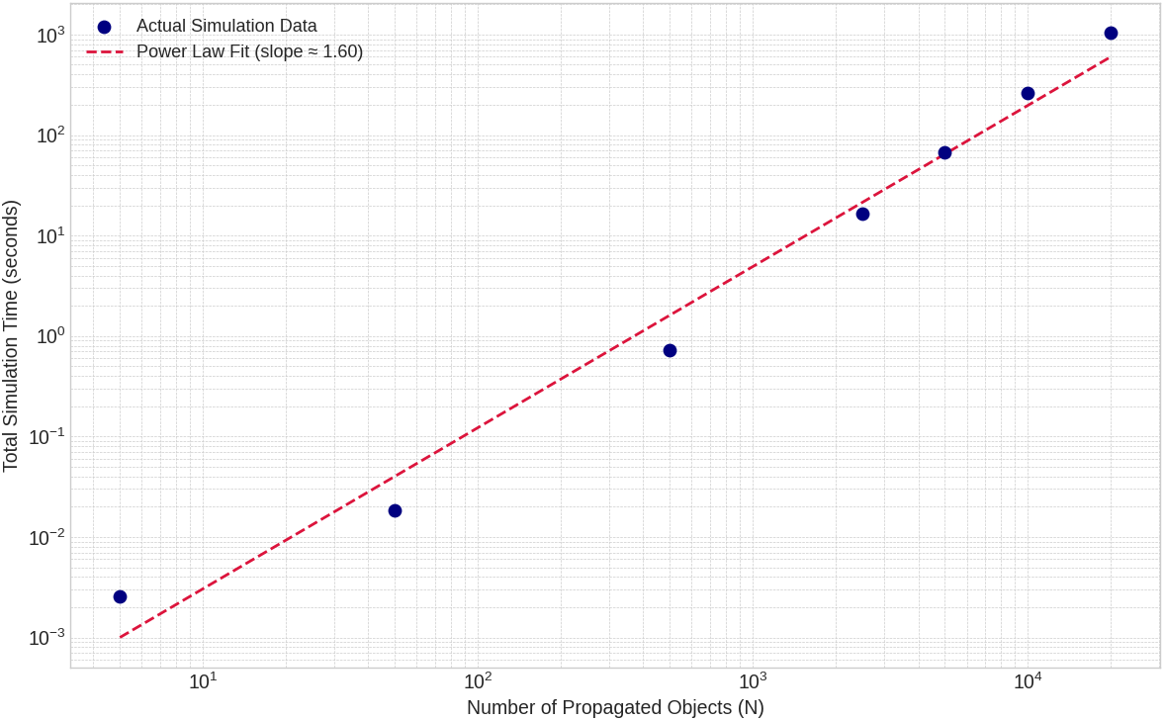
\includegraphics[width=1\linewidth]{scalability_plot.png} 
\caption{Log-log scaling performance tracking object population size against numerical integration processing time in seconds.}
\label{fig:power_law_fit}
\end{figure}


\section{Conclusion}
This accelerated research proposal establishes a structurally consistent, high-fidelity methodology designed to address the scalability and physical limitations of contemporary orbital debris forecasting tools. By mathematically integrating a second-order Strang splitting sequence with advanced neural network surrogates, the proposed framework achieves sub-kilometer physical tracking accuracy while significantly decreasing total computational runtime latencies. The successful execution of this 2-year doctoral plan provides the astrodynamics community with a robust mechanism for proactive space traffic management, securing long-term sustainability across congested orbital regimes.


\section*{Funding Sources}
This doctoral research is technically and financially supported by the Research Group in Efficient Energy Management (GIMEL) at the Universidad de Antioquia, alongside the Aerospace Engineering program from the Department of Mechanical and Aerospace Engineering.


\section*{Acknowledgments}
The authors express their gratitude to the Faculty of Engineering at the Universidad de Antioquia for providing the processing infrastructure required for large-scale parallel simulations. Additional acknowledgment is extended to Odyssey Space Research in Houston, Texas, for providing high-fidelity baseline technical consulting profiles throughout the design of the numerical validation loops.

\bibliography{references}
\bibliographystyle{ieeetr}

\end{document}